\chapter{Documentation}
%\addcontentsline{toc}{chapter}{Appendix - Documentation}
\addtocontents{toc}{\protect\setcounter{tocdepth}{0}}
This section will provide a guide to using our application and insights on the written code. Fist we will introduce the application to an end user. Then we will go into details about the structure of the code and used data.
\section{User Documentation}
This part of the documentation is focused on the end user, in this case, player. We introduce controls of the application and detail the possibility to adjust the game world.
\subsection{User interface}
Here, we provide the list of parameters and key bindings needed to control our application.
\subsubsection{Parameters}
The application provides only one console parameter. It is {\tt -d}, and it enables debugging information to be rendered. In other words, it draws the collision shapes and bounding boxes around the objects.
\subsubsection{Keyboard input}
Keys can be pressed simultaneously and also held down instead of multiple presses. The bindings are:
\begin{itemize}
\item W/S: pitch down/up
\item A/D: roll counter-clockwise/clockwise 
\item Q/E: yaw left/right
\item Z/X: speed up/slow down
\item Space Bar: shoot or unpause
\item P: pause the game
\item ESC: quit the game
\end{itemize}


\subsection{Input data}
\label{sec:data}
To allow the user to easily change the game world without the need of recompilation the input text file describing the whole setting is provided. The mentioned file is located in {\tt media/world.cfg}. 
\subsubsection{{\tt world.cfg} format}
We will show that the structure of the data is straightforward and therefore we have chosen not to use XML or any other standardised format. The file is interpreted by lines. Each line represents one in-game entity. First three lines have special meaning, and the rest are destructible objects. Inside the line, we use semicolons as a separator between data items.

The \emph{first line} describes the sky-box, it is formed of 6 images in given order: top, bottom, left, right, front, back; relative to the starting viewpoint. 

All other lines use same nine data items. Those are object model, texture, position (3 coordinates), scale (3 numbers, one for every axis) and mass. Every number is used as a floating point number.
The second line describes the ground. Currently, the ground is generated as a solid cube with 1x1x1 size. Therefore model file is not needed. The third line is a description of our controlled vehicle. Beginning with this line, the texture file is an optional parameter and can be left blank. Bellow, we can see an example file.

\begin{centering}
\begin{Verbatim}[frame=single,numbers=left,xleftmargin=5mm]
top.jpg;bottom.jpg;left.jpg;right.jpg;front.jpg;back.jpg
;grid.jpg;0;-15;0;1000;10;1000;0
fighter.3ds;;0;20;0;0.5;0.5;0.5;1
building.obj;;-20;-11;-30;2;2;2;500
pyramid.obj;;50;-11;-100;5;10;5;800
...
\end{Verbatim}
\end{centering}
The zero mass means that the object is static and does not move.

The input formats are limited to the support of \emph{Irrlicht}. The detailed list of supported object and texture formats can be found on \emph{Irrlicht} web page~\footnote{http://irrlicht.sourceforge.net/?page\_id=45\#supportedformats}



\section{Implementation details}
This section provides insights on the code from a programmers point of view. We will not focus on algorithms here, as we already did that in \cref{chaptImplementation}. The main focus here is on data representation and division of code into multiple modules.

\subsection{Data representation}
As a result of using multiple libraries for a multitude of tasks, we have to deal with a lot of different data representations of the same objects. 

We will introduce the data structures that are used to represent one in-game object for multiple purposes. We can see how different data types are converted in~\cref{fig:conversions}.
\begin{description}
\item [{\tt btRigidBody}] is a class \emph{Bullet physics} uses to hold an information about a rigid collision object. For us, most important part of the body is a collision shape.

The collision shape can be of multiple types. Most notably a convex hull or a primitive geometric shape, a triangular mesh or a compound shape. We need the collision shape to be as close to a visual mesh as possible. Because calculating collision between triangular meshes is not implemented in the \emph{Bullet physics} and would be too costly. The compound shape is the only option.

One more parameter of {\tt btRigidBody} to consider is mass. Bodies with mass set to zero (or negative value) are considered static objects and do not move. Bodies with mass react to gravity and other external forces, their centre of gravity is set to their respective origin of local coordinates. This poses a problem when the origin is not inside the object. The solution is to manually translate the mesh, vertex by vertex, to the origin.

\item [{\tt irr::scene::ISceneNode}] is a representation of a graphical object in the \emph{Irrlicht engine}. It is an abstract class instantiated into multiple types of graphical objects, \eg lights, cameras, animations, particle systems. We are using {\tt irr::scene::IMeshSceneNode} for our objects. The mesh information in {\tt irr::scene::IMeshSceneNode} is stored in {\tt irr::scene::IMesh}. 

\item [{\tt irr::scene::IMesh}] stores the mesh information in multiple mesh buffers. Each buffer has an array of vertices and an array of indices. Every index in the array of indices refers to one vertex. However, we found out that not every vertex is referred to, and therefore valid. Indices divided into consecutive non-intersecting triples form a triangular face of a mesh. 

The fact that the mesh is split into multiple mesh buffers and the fact that every face in each mesh buffer must be complete needs to be addressed when converting the data. If we have two neighbouring faces and both are stored in different mesh buffer, their common edge is stored twice. When converting to {\tt CGAL::Nef\_polyhedron\_3}, the duplicity in edges bans us from copying the mesh face by face and requires filtering, because overlapping geometry is not allowed in {\tt CGAL::Nef\_polyhedron\_3}.

\item [{\tt CGAL::Nef\_polyhedron\_3}]

\item [{\tt gg::MObject}] is our class designed to unite the data of one in-game object into one object in the code. It includes {\tt irr::scene::ISceneNode}, {\tt CGAL::Nef\_polyhedron\_3} and {\tt btRigidBody}. We also implemented mechanism ensuring that upon deletion of an object, its parts are first removed from their respective engines, then deallocated and at the end {\tt gg::MObject} itself is destructed.

\end{description}

\begin{figure}
        \centering
        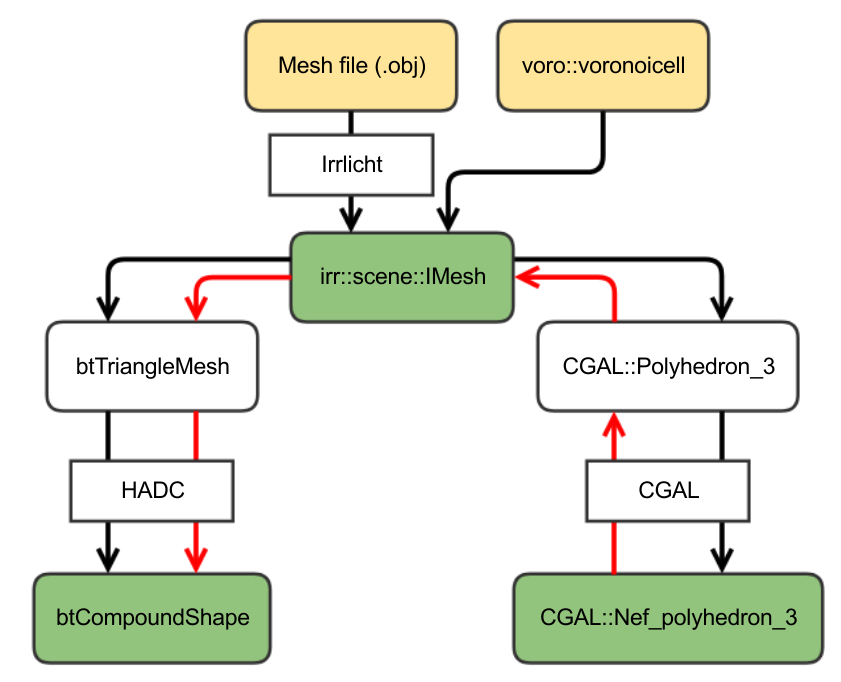
\includegraphics[width=\textwidth]{img/conversions}
        \caption{Data conversion diagram. Input formats - yellow, required formats - green. Black lines show used conversions, red lines show required process after a change of the shape of an object. Rectangles signify the library used to make the conversion, if none a member function of {\tt gg::MMeshManipulators} is used.}
        \label{fig:conversions}
\end{figure}

\subsection{Modules}
In this section, we describe the functionality of each program module. Third party software will not be described here. It can be found in \cref{chapt:technology}. Interactions between modules are described in \cref{fig:modules}. \emph{Irrlicht Engine} is not present in the diagram because we do not logically depend on using this engine. Every module is implemented in a file with the matching name as a class with the same name prefixed with letter M (Object Creator can be found in file ObjectCreator.cpp and is implemented as class {\tt gg::MObjectCreator}). Every component of our part of this application is located in namespace {\tt gg};

\begin{figure}
        \centering
        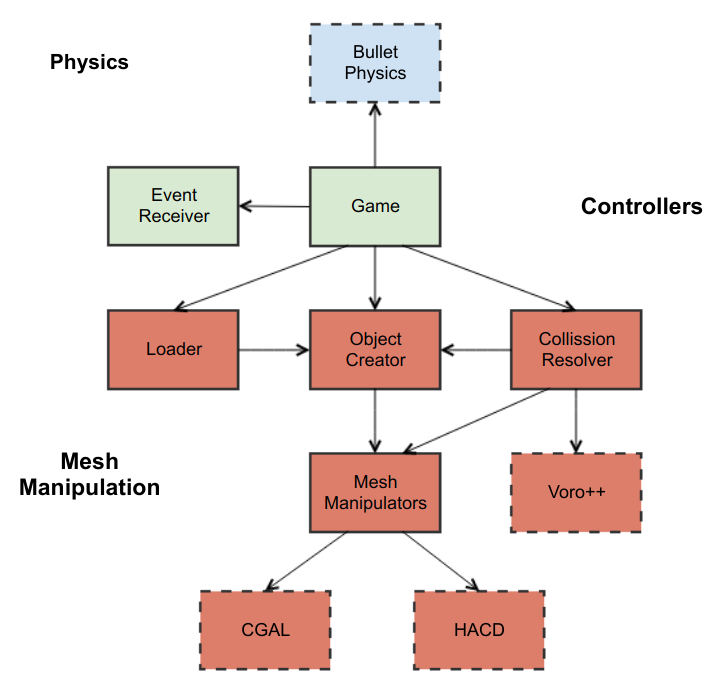
\includegraphics[width=\textwidth]{img/objectmodel}
        \caption{Software architecture shown on diagram of relationships of program modules. Third party software is highlighted in dashed rectangles.}
        \label{fig:modules}
\end{figure}

\begin{description}
\item[Game]
This module holds {\tt gg::MGame} class which is the core of the application. The communication with the physics engine,  the graphical engine and mesh manipulation parts of the software is managed from here.

\item[Event Receiver]
This class is an implementation of {\tt irr::IEventReceiver} from Irrlicht engine and it is used to read the user input.

\item[Loader]
The Loader is a class only used for initializing the application. It parses the data describing the game environment from the given file, constructs the objects with the help of {\tt gg::MObjectCreator} and returns the set of constructed objects.

\item[Object Creator]
We use this class as a Builder pattern in order to initialize the data contained inside {\tt gg::MObject} ({\tt CGAL::Nef\_polyhedron\_3, btRigidBody, irr::scene::ISceneNode}).

There are three member functions allowing us to create {\tt gg::MObject}s  with different behaviour from the same set of input parameters (see \cref{sec:data}). We can achieve a destructible object, an indestructible object with box collision shape and a rectangular indestructible object without input mesh. Those functions are exclusively used at initialization as they generate a new set of member variables, and their parameters come in a text form.

Two more kinds of objects can be created a projectile that is shot from the given position with the given impulse and a destructible object with temporary collision shape (sphere shaped). Because the object with temporary collision shape is constructed while the game is being played and construction of {\tt CGAL::Nef\_polyhedron\_3} can take a longer time, it requires to have the {\tt CGAL::Nef\_polyhedron\_3} given in parameter. Indestructible objects do not require {\tt CGAL::Nef\_polyhedron\_3}  and therefore the shooting is not limited by their construction time.

\item[Collision Resolver]
After every collision, Collision Resolver decides what to do with it, and in the case of destruction, takes care of the whole process. To process the collision, {\tt gg::MCollisionResolver} owns both Mesh subtraction and Convex Decomposition threads. The Voronoi cell generation is also done in this module. Collision resolver heavily relies upon Mesh Manipulators utility functions because many data conversions are happening in here.

\item[Mesh Manipulators]
Mesh Manipulators provides set of public static functions. Because different libraries are used for physics simulation, rendering and geometric manipulation, those functions provide means for converting data between different formats.
\end{description}